%% LaTeX2e class for student theses
%% sections/content.tex
%% 
%% Karlsruhe Institute of Technology
%% Institute for Program Structures and Data Organization
%% Chair for Software Design and Quality (SDQ)
%%
%% Dr.-Ing. Erik Burger
%% burger@kit.edu
%%
%% Version 1.2, 2016-09-20

\chapter{Introduction}
\label{ch:Introduction}

%%%%%%%%%%% Something something present day communications, bandwidth, etc.
With the proliferation of mobile communications, the amount of internet users has grown exponentially since 1993 to a staggering amount of 2.95 billion users, corresponding to 40.7\% of the world population as of 2014 \cite{ITUinfo15} with an estimated total market penetration of 46.1\% by the end of 2016 \cite{ILSinfo16}. As more devices and users are added to the network, the need for technologies that can support higher data rates has become a key element in the design of server applications and the hardware that supports them. 
\par\medskip
In order to sustain the growth of telecommunication data rates, it is necessary to scale the computation nodes, processing units, datacenters, and most importantly, the links between the interconnected devices. As the bandwidth requirements are increased to handle more users, the volume of data between servers must also be scaled, and the distances that data must traverse without losses become a significant limitation of copper interconnects; Additionally, the Shannon theorem connects the data throughput to the bandwidth of the channel, based on its physical limitations, such as latency and power efficiency. Thus, in order to achieve low power consumption while increasing the data rates, the employment of optical communications has had a great impact in achieving the ever-demanding data traffic in modern short-haul telecommunications. Optica communications feature higher data rates, larger bandwidths and higher noise immunity compared to electrical interconnects, with the additional advantage of reduced complexity of the cabling solutions.
\par\medskip
%$\lasnotas{I still need to connect the speed of data with why optical devices are important}.
%By itself, silicon is an excellent semiconductor candidate for optical communications: Transparent in optical communication wavelengths; highly tunable by doping; and thermally and mechanically stable.
The integration of optical communications to the current state-of-the-art computation nodes demands the use of the existing standardtechnologies in the industry, such as \textbf{silicon-based microelectronics processing}, effectively aligning the well-known processes of microelectronics with new developments in the field of photonics. The concept is extended to the so-called \textbf{silicon photonics}, where photonic platforms are developed using silicon as the core semiconductor component, which provide the technological framework for optical communications compatible with the current microelectronics processing and manufacturing. Silicon is the most widely used semiconductor in the manufacturing of electronics, due to its versatility, availability, low cost, electrical, mechanical and optical properties and industry maturity. Nonetheless, not all of its properties, especially in the optical range, are optimal: silicon is an indirect semiconductor, and possesses a very weak stimulated emission (due to poor radiative band-to-band recombination emission \cite{PavesiSi06}), make it unsuitable as a light emitter, and a lacking an intrinsic electro-optic effect (due to its centrosymmetrical crystalline structure) make it unsuitable for high-speed modulation. Additionally, silicon has better absorption in the UV range than in the deep IR (making it unsuitable for most modern optical communication standards). Thus, additional elements must be integrated to the silicon photonics platform in order to achieve the desired high data rates. 

Since the invention of organic light-emitting diodes (OLED) by Tang and Van Slyke in the 1980s, research in the field of organic semiconductors has flourished and developed substantially \cite{SoOrga09}. Of main importance to the present work are organic semiconductors that can be externally poled leaving a long-lasting polarizability in the molecules conforming the organic compound, making it a suitable electro-optic material, which also has the advantage of possibly enabling direct deposition techniques (such as spin-coating or doctor blading) removing some complexity to the formation of a stack-up formation by crystal growth or lithographic processes, for example. The electro-optic effects are the main focus of study in the present work, by using a silicon-organic hybrid (SOH) platform to provide an alternative to inorganic semiconductor modulation. 
\par\medskip
In the field of microelectronics, the integration process is relatively straightforward, due to the well-established building blocks used in electronic circuits: Resistors, capacitors, inductors and transistors. The building blocks can be easily manufactured by using different materials, such as metals, semiconductors and insulating materials, and thus very diverse electronic circuits can be built and designed for very complex integrated circuits in a single packaged device. In the case of photonic integration, the process must also have basic building blocks which manipulate light such that a specific function is achieved. The photonic building blocks include the light sources, optical amplifiers, optical modulators, polarization circuits, multiplexers, filters and couplers \cite{SmitSiPh14}. Photonic integration may require the use of different platforms in order to exploit the performance of different technologies that could not be otherwise monolithically grown, due to atomic incompatibilities or inherent integration complexity. These devices are the so-called multi-chip modules (MCM), which feature different technologies integrated into a single common carrier. Much like their electrical counterpart, the devices have to connected to each other in order to process light. That means that light must be guided through the connected devices, by means of optical waveguiding or free-space propagation of light. The \textbf{photonic wire bond} (PWB), is of special interest in the context of this thesis as it is the photonic element that connects two optical devices in which light propagates and has small dispersion and low losses with the benefits of the optical range bandwidth inherent in waveguiding. PWBs have the advantage over free-space optical coupling of requiring no active beam alignment, since the PWB is directly attached to the optical device; very stable operation over several temperature ranges; low losses; broadband transmission; and scalability for large-scale device deployment \cite{LindenmannPWB12}. 

%No idea why this is here!
%In the classical model for computing architecture, the transmission, processing and interpretation of information (\emph{software}) has to be done in a physical device (\emph{hardware}). With increasingly complex interconnections and data formatting, the relation between hardware and software has drifted apart from the approach given by Von Neumann in the 1960s into a more complex paradigm. Kirischian \cite{RecCompSysEngKirischian16} distinguishes the role of \textbf{components} as hardware and software, leading to the concept of \textbf{hardware platforms}, which are hardware components designed for a specific implementation.

%The photonic platform building blocks of interest for an optical transmitter consists of one or more of the following elements\cite{USBOpto16}:

%\begin{itemize}
%\item The \textbf{laser} is the optical element that generates the light that is transmitted through the communication channel. The most common communication channel for optical communications are optical fibers.
%\item The \textbf{modulator} is the element that shapes the optical signal (carrier) with the data to be transmitted into the communication channel. The modulator can be a simple, single modulator for on-off keying (OOK) or a group of modulators with more dense data format, such as quadrature phase shift keying (QPSK), by exploiting in-phase and quadrature schemes.
%\item The \textbf{photodetector} is the component that receives the optically modulated signal and correspondingly converts it to an electrical signal. Detection can be done coherently or incoherently depending on the bandwidth availability and the expected signal-to-noise ratio (SNR). 
%\item The \textbf{waveguides} that propagate the light across the different photonic circuits for its manipulation. 
%\end{itemize}


\par\medskip
\begin{figure}[!ht]
\centering
  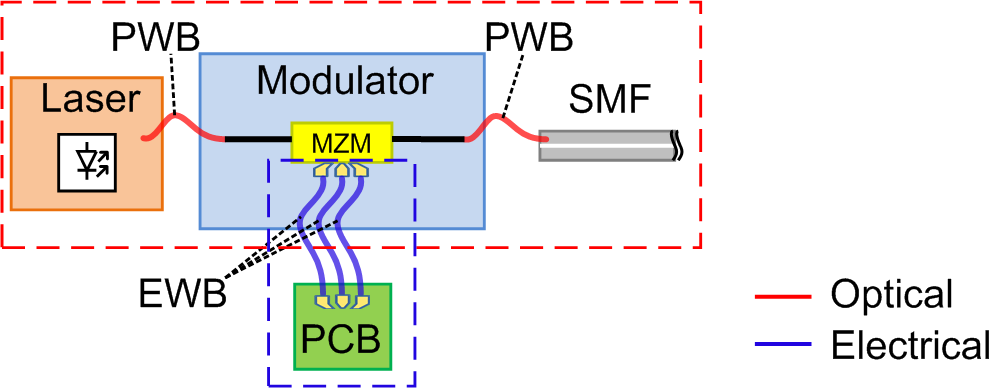
\includegraphics[width=0.7\textwidth]{visio/Schematic_Concept}
  \caption{Schematic representation of optically- and electrically-packaged transmitter. A laser source is connected through photonic wire bonds (PWB) to a MZM modulator that launches the modulated signal through another PWB to a single mode fiber (SMF). The modulator is driven by electrical wire bonds (EWB) to a printed circuit board (PCB) with RF connectors. The dashed outline shows the optical packaging (in red) and the electrical packaging (in blue).}
  \label{fig:SCH_Concept}
\end{figure}

Figure \ref{fig:SCH_Concept} shows the schematic concept of a fully-packaged transmitter. Without loss of generality, the laser, modulator and output single mode fibers are optically packaged into a single common carrier by using PWBs as optical waveguiding elements. In order to electrically access the device without the need of microprobes, which tend to damage the extremely sensitive devices to mechanical vibrations and external manipulation, an additional electrical wire bonding (EWB) can be added to electrically package the transmitter by means of BNC connectors onto a printed circuit board (PCB) and thus enabling testability and further completely packaging the device. The end product that can be achieved are the so-called active optical cables (AOC)\footnote{https://www.finisar.com/active-optical-cables}, which feature transmitters and receivers optical-based interconnection network. The objective of this master thesis focuses on the optical integration and packaging of the transmitter, specially focused on the process flow steps to achieve a homogeneously-operating transmitter.

%Only the optical packaging is of interest in the framework of this master thesis.

\par\medskip

The master thesis is separated into four main components:
%\footnote{pronounced ``heex-cel'', as its equivalent counterpart VCSELs or ``veex-cels''.};
\begin{itemize}
\item A \textbf{theoretical framework} is provided covering the most important elements that comprise an optical transmitter: The silicon-organic hybrid (SOH) modulator, its theory of operation and important figures of merit; the free-form waveguiding element or photonic wire bond (PWB) and its fabrication principle; and finally, the most important aspects of integrated modulators, such as the light source chosen, featuring a brief introduction to the operation principle of the horizontal cavity surface emitting laser (HCSEL), as well as the optical path losses which provide the most important figures of merit to determine the performance of the optically packaged transmitted.
\item The \textbf{integration process} is described thoroughly, including the variations and discoveries found throughout the experimental procedures. Some elements of past theses are revisited regarding the integration process and the modifications required for a stable process are outlined.
\item The \textbf{data transmission experiment} is used to demonstrate that the multi-chip modules produced are operating adequately. The setups are thoroughly described and the results obtained are discussed. The data transmission experimental setups are described for direct and coherent detection cases. 
%contains the laboratory work and results obtained during the master thesis, including the characterization of the HCSELs; the fabrication process of the transmitter, including the fiber mounting and materials used for the integration; the writing process of the PWBs; the activation of the modulator electro-optical material; and the characterization of the optical modulator. 
%\item The \textbf{discussion} section provides some insights on the obtained results and the thorough analysis of the obtained results. In some cases, the discussion leads to additional laboratory procedures for confirmation of some hypotheses, so some laboratory results are also mentioned here, including the thermal performance of the HCSEL and alternative processing schemes of the transmitter elements.
\end{itemize}

Finally, the outlook of the project and the conclusions are discussed in brief.

%% -------------------
%% | Example content |
%% -------------------


%% --------------------
%% | /Example content |
%% --------------------